% !TEX TS-program = xelatex
% !TEX encoding = UTF-8 Unicode 

% \documentclass[AutoFakeBold]{LZUThesis}
\documentclass[AutoFakeBold]{LZUThesis}
\usepackage{multirow}
\usepackage{threeparttable}
\CTEXsetup[name={第,部分}]{chapter}
\lstset{
language = MATLAB,
backgroundcolor=\color{white},   % choose the background color; you must add \usepackage{color} or \usepackage{xcolor}  
basicstyle=\footnotesize,        % the size of the fonts that are used for the code  
breakatwhitespace=false,         % sets if automatic breaks should only happen at whitespace  
breaklines=true,                 % sets automatic line breaking  
captionpos=bl,                    % sets the caption-position to bottom  
% commentstyle=\color{green},    % comment style  
% deletekeywords={...},            % if you want to delete keywords from the given language  
% escapeinside={\%*}{*)},          % if you want to add LaTeX within your code  
extendedchars=true,              % lets you use non-ASCII characters; for 8-bits encodings only, does not work with UTF-8  
frame=shadowbox,                    % adds a frame around the code  
keepspaces=true,                 % keeps spaces in text, useful for keeping indentation of code (possibly needs columns=flexible)  
keywordstyle=\color{blue},       % keyword style  
% language=Python,                 % the language of the code  
morekeywords={*,...},            % if you want to add more keywords to the set  
numbers=left,                    % where to put the line-numbers; possible values are (none, left, right)  
numbersep=5pt,                   % how far the line-numbers are from the code  
numberstyle=\tiny\color{gray}, % the style that is used for the line-numbers  
rulecolor=\color{black},         % if not set, the frame-color may be changed on line-breaks within not-black text (e.g. comments (green here))  
showspaces=false,                % show spaces everywhere adding particular underscores; it overrides 'showstringspaces'  
showstringspaces=false,          % underline spaces within strings only  
showtabs=false,                  % show tabs within strings adding particular underscores  
stepnumber=1,                    % the step between two line-numbers. If it's 1, each line will be numbered  
stringstyle=\color{orange},     % string literal style  
tabsize=2,                       % sets default tabsize to 2 spaces  
% title=signalAnalysis.m           % show the filename of files included with \lstinputlisting; also try caption instead of title  
}  

\begin{document}
%=====%
%
%封皮页填写内容
%
%=====%

% 标题样式 使用 \title{{}}; 使用时必须保证至少两个外侧括号
%  如: 短标题 \title{{第一行}},  
% 	      长标题 \title{{第一行}{第二行}}
%             超长标题\tiitle{{第一行}{...}{第N行}}

\title{{职业生涯规划之我的成长史}}



% 标题样式 使用 \entitle{{}}; 使用时必须保证至少两个外侧括号
%  如: 短标题 \entitle{{First row}},  
% 	      长标题 \entitle{{First row}{ Second row}}
%             超长标题\entitle{{First row}{...}{ Next N row}}
% 注意:  英文标题多行时 需要在开头加个空格 防止摘要标题处英语单词粘连.

\author{\CJKfontspec{楷体}李文涛}
\major{电子信息基地班}
\college{320200928101}
\grade{2020级}



\maketitle
\frontmatter

%中文摘要
\ZhAbstract{
    本文首先以AMI码为对比对象介绍$\mathrm{HDB_3}$的由来,简略介绍该编码方案的优缺点,
    接着利用MATLAB进行编程,完成对原数字信号序列进行$\mathrm{HDB_3}$编码
    以及后续对信号的频谱分析,对编码
    时频域分析进行谱图可视化,并同时分析其在其传输速率和频谱利用率上的特点。
    最后根据其频谱特性分析其应用价值。
}
{优缺点,MATLAB,时频域分析,应用分析}


%英文摘要
\EnAbstract{This paper introduces the advantages and advantages of $\mathrm{HDB_3}$, 
and then uses MATLAB to program,
 complete the $\mathrm{HDB_3}$ encoding of the original digital signal sequence and the subsequent spectrum analysis of the signal, 
 and the spectral diagram visualization of the encoding time frequency domain analysis, 
 and analyze its characteristics in its transmission rate and frequency utilization.
 Finally, its application value is analyzed according to its spectral characteristics.
    \fontspec{Times New Roman}}
{Advantages and disadvantages, time frequency domain analysis, application analysis}

%生成目录
% \tableofcontents
% \addcontentsline{toc}{chapter}{目录}
% \thispagestyle{empty}


%文章主体
\mainmatter

\chapter{过去的碎片}

\section{上初中之前的那些日子}

\subsection{自立的生活}

我出生在一个教师家庭,父母都是高中老师,小时候我经常一个人在家,
摆弄着手上的玩具,消遣着时光。印象比较深的是我和外公在一起的日子,当时我外公会带着
我和同事打交道在一起玩(当时外公在高中后勤工作),那段日子不能说无忧无虑,但
那段时光是我珍贵的童年记忆。

小学没什么特别的记忆,记忆最深的可能就是小学门口等父母来接的场景了,由于父母工作的关系,
我常常是我们学校门口最后离校的几个人之一。为了消磨这段无聊的时间,我常常会带些
小玩意来和同学们一起玩,当时就有一种风气,想起来有点好笑,小学里流行玩的东西经常
就是我在等父母来玩的那些小玩意——卡片啦、弹珠啦。

说起来还有一次父母两人工作得太忙,以至于忘了接我这件事。当时下着雨,天也已经
黑了,空气凉飕飕的,周围也只有时不时骑着电动车路过的路人,我躲在一个路边的
公交站台避雨等着父母来接,有一个过路的阿姨发现了我,主动问我为什么在这,我回答父母还没来,
她便借我手机给家里打电话,父母这才来把我接走。

那段时间父母时常不在家,我干什么基本上是绝对自由的,父母也不会过于深究我的学习,我便花了
大量的时间在看课外书和看电视上,也许就是那些时候看的东西初步构成了我的三观,
让我迫切地想去更多地了解这个世界。

\subsection{朋友的概念}
也许是受独立生活的影响,我对朋友的观念一开始就有着这样的理解:推心置腹、无话不谈。
印象比较深的有之前的邻居家的两兄弟,当时我家住在四楼,他们在三楼,我们经常在一起玩,
虽然年龄段不同,但我们却还是能玩到一起,小时候玩乐时的愉快也大多是和朋友在一起的
记忆。

正是由于这个从小就形成的朋友的观念吧,我身边的朋友一直不是很多,但我很满足,
因为在我看来,我的朋友是真正能够接受我的人,正如那句话所说,“人生得一知己足矣”,
虽说不至于达到“知己”的程度,但也算是“共情”的对象。这影响了我今后的交友标准和交友范围,
也导致在别人看来,我并不是很合群,在今后的生活中虽说有所改善,但朋友的定义始终没有什么
改变。

\subsection{个人性格的养成}
我想由于小时候环境和书籍的影响,我不太爱与人交往,准确来说,是没有意义的交往,
我认为没有意义的交往是在浪费时间,这也导致我自己的性格在很多人看来很烂:拒绝交流、
目中无人、“孤芳自赏”。但正是因为这样,我认为我省去了很多不必要的交往,因此有了
更多的时间去来了解世界。

受当时部分书籍的影响,我的心智成熟得及其迅速,以至于现在的我都对记忆中我当时的
一些观念给予肯定,在周围的人不能理解我的心思的时候,我便更加沉浸于自己的“舒适圈”。
有一个词叫做“中二病”,当时的我也许就给人那样的感觉吧。

\section{初中——心智急速成熟的时期}

\subsection{学习之路}
进入初中,在这段时期,除了学习之外好像也没有什么值得一提的事情,由于地域和家庭的原因,
从小就被灌输学习是唯一出路的我在初中就开始和“刷题”有了不解之缘,应试教育和我当时的三观
起了不小的冲突,“学习”一次在我的心理就变成了一种让我困惑的名词,
一方面,我喜欢学习和探索新的知识,而另一方面,我学到的知识用一张充满着套路的试卷来检测,
这使我感到不解和无奈。

同时在这时我对大学有了一定程度上的向往,想象着大学能够真正学到具有完整体系和用于实际
的知识,为此我即使对一张张套路的试卷抱有不满,但还是接受着并保持着成绩。

\subsection{个人性格的定型}
上初中时,自己已经具有了一定的判断能力,对周遭环境变得更加敏感,喜欢带着审视的眼光
去看待人和事。当时学习的压力还不是很大,留给我充分遐想的时间,那时我总会一个人陷入对
社会和人生的大思考,最终在不知不觉中完成了我的性格的定型——避世、随性而为,听起来
有些消极,但是其实并非如此,实际上我对此的解释就是听从自己的选择、不为自己的选择后悔,
做最真实的自己。

这可能是周遭无法正确地认识我,我自己对其他事物感到失望并坚定实现自己的目标而导致的,
实际上这种想法确实让我生活地十分洒脱和开心,以至于后来高中的语文老师评价我“活得像个仙儿一样”,
当然这既不是贬低也不是褒奖,是对我生活状态的一种评价。把一切东西看得看清,同时也看得
太轻。这是我尝试向别人传达思想但屡次失败的妥协。也许,这是我的叛逆期也说不定。

这个时期,我接触了许许多多与我思想共鸣的事物——电影、音乐、书籍亦或是被称为第九艺术的游戏,
我在这些形形色色的事物上感受到了制作者寄托的感情,我也很乐意乘醉其中,享受这片精神家园。
有时去聆听社会经济低迷时形形色色的人心中的呐喊,又有时体验即使不被人理解但依旧坚持本我的生活,
亦或体验背负责任踽踽独行的孤独。这些思想的碰撞使我总是悲观地面对外界事物,
相信“正因目睹过黑暗的无情,才会知晓光明的珍贵”。

\section{高中——夹缝中生存}
\subsection{考学的压力}
我出生在河南,众所周知,这是一个高考大省,但,它所不为人知高考压力,也许只有亲身体验过后
才有资格评价吧。正巧,近期有“小镇做题家”这个形容词,我觉得它是一个非常贴切的称号,
我所在的高中,高中三年的前两年会把所有的科目结课,部分科目甚至是一年半,接下来的时间分配
就很简单,做试题、做试题、“做到进入高考考场”,高中三年都是在持续高压中度过,每天三点一线,
早上5点到晚上10点,除了解决必要的生理需求,其余时间就是在学习,每顿吃饭的时间都要压缩至20分钟
以内,在去买饭的路上快速奔跑,为了以免去的太晚在排队时浪费时间。有的时候还是会懈怠,也许这是
因为这段时间是每天宝贵的唯一能从学习中“逃避”出来的时间吧。

那时的学校对于我们来说就如同“集中营”一般,按部就班地进行着高考机器的加工,如强心针一般的口号在校园里
无处不在,“两眼一睁,开始竞争”,伴随着每天的铃声,拖着还没完全苏醒的身体,喊着规定的口号进行着所谓
“衡水式”跑操,飞奔在去餐厅的路上还要时时刻刻想着还未做完的题目,在一科接着一科的作业中寻找夹缝喘气,
一次又一次的考试让人麻木,而一次次的分数时刻都能成为压垮我们的最后一根稻草。

然而,我们最后得到了什么呢?虽然老师们经常以“考察你们的学习能力”为说辞来告诉我们学习的意义,但那
也只是借口,又有谁不知道是为了在高考中多得一分这一骨感的事实呢?高考作为多年来判断学生是否
优秀的标准,其合理性、正规性、公平性不言而喻,但又是什么造成了这一切呢?人口基数、教育资源的差异?
又亦或是其他,不论是什么原因,造成的现状就是我所看到的近乎病态的“唯分数论”,我痛恨自己,恨自己
将时间用于研究每道题的答法做到步骤尽善尽美、用于练习字体哪怕在哪里能够让老师多给一分,而不是
用这些时间去接触我感兴趣的电信技术,为大学的到来做好预习。我明白在百万考生中奋力得到一份
满意的通知书并非易事,但同时也对摆在眼前的题海无能为力,那种无力感就像你奋力去击打现实,但
又好像打在棉花上一样,毫无作用。

在高考出分的那晚,我也像众多的高中生等着分数的公布,当知道那个不尽人意的分数时,我的心情
十分复杂,有质疑、也有悔恨。那是我高中三年考得最差的一回,当我第一次成为为高考成绩发愁的一个
家庭的中心,我感到茫然无措,家里人对我的分数不满意,想让我去复读,我拒绝了。
我知道,我可能无法再在那种环境中撑过一年。明白我意思的父母就不停地帮我寻找合适的大学,
第一次看着父母那样的焦急,我的内心也经受着煎熬。最终在一个母亲的同学那里得到了对兰州大学的肯定,
选择来到西北这片土地进行我的大学学习生涯,现在看来,这也许是最好的选择了。


\subsection{精神的共鸣}
正如之前所说,我认为“正因目睹过黑暗的无情,才会知晓光明的珍贵”,我在高中结识了富有个性、志同道合
的朋友,感谢有他们,才能使我的高中生活不尽是令人压抑的灰,也有令人愉快的彩。我们在一起聊
共同的兴趣,被书中的情节触动心弦,在一起讨论游戏的设计和文案,吐糟着番剧里出其不意的剧情,总想
着那段时光延长,再延长,能多一些就好了。

在高中的时候,有一部日本的轻小说作品令我印象深刻,因为书中的主角令我心驰神往,为什么呢?
书中的他,给人一种边缘的感觉,“爱好是观察人类”,不喜与人交流,
十分擅长“读空气”,虚伪的人际关系令他作呕,但这样的他也会在别人需要时伸出援手,
以自己的方式去帮助他人,甚至以一种“自残”的方式去解决问题,
将问题的矛头全部引向自身,即使不被人理解,背负着误解,
但他知道,这样才是最好的,用自己的不幸去维持多数人的关系,换取大家的快乐,这就是他的正义观。
正是这样的他,有着几个真正理解他的人,会在他“自残式”解决问题时告诉他“有人会因你而心碎”,会
伸出援手向大家介绍这样一个古怪的人。那种人与人之间的羁绊,是我梦寐以求的真物。

虽然没有小说中那这过于理想的人际关系,但我十分满足于自己的生活,我喜欢自己决定的生活,
“我们口中所说的日常,也许是连续不断奇迹的发生”,做自己,并且有支持自己的人,快乐莫在于其中了。


\section{部分小结}
从小自立的生活培养了我独立思考的能力。
小时候的我便十分珍惜朋友,对朋友的定义也较为严苛。
养成了与他人一般不会敞开心扉的性格,但对于真正的知己无话不谈。
珍贵的高中回忆,让我在精神上得到了肯定,对人生充满自信。也养成
了看待事物不予深究,坚持自己的处事风格。
初中开始感受到学习的压力,接触到由学习带来的竞争。
通过高中三年的努力,给不完美的高考画上了句号。

\chapter{现在的自己}

\section{大学新天地}

\subsection{基本独立的生活}
离开家乡,我的内心是雀跃的,第一次获得了真正意义上的自由,拥有属于自己的独立空间,也不会
受到家里人过于频繁的问候,在新的校园,我结交了新的朋友,认识到了许许多多我感兴趣的新生事物,
可以学到自己感兴趣的知识,也许会有点难学,但我感到这些知识才是我想要的,是那种能够在我了解世界
这方面帮助我前行的有力伙伴。

但与之相伴的,还有更加骨感的人际关系,都说“大学小社会,社会小大学”,
人总会在和别人交际时多加一层防备。由于目标的一致,总会
引起形形色色的勾心斗角,不免有些为了利益趋之若鹜的人采用不太光彩的手段。但这对于我来说都
无法在我心中造成波澜。
因为我的处事风格就是顺其自然,该放手的决不挽留,该挽留的绝不放手,不愿与之较劲的我,没必要
受到这些人的影响而改变自己,只要走自己的路就好了。

\subsection{大学生活的学习}
平心而论,进入大学之后,虽然有接触新知识的喜悦,但更多的还是让人感到不适应,因为对于我来说,
那些东西都很难,由于和高中的应试不同,大学的东西需要自己去探索、去深究才能获得回报,看到
周围同学都学得得心应手,我对自己也产生了怀疑,在经过了开始的“阵痛期”后,我逐渐掌握了自己
的学习方法。

回过头来发现,大学的时光是那么的紧张,转瞬即逝,需要你对自己的状况有完整的把控,
自己要学会利用时间去反复理解课本的内容,只凭课堂的理解就能学会实在对我来说是强人所难。
有过高考过后不顾一切报复式的娱乐,有过学不会后摆烂的妥协,也有自己在台灯下整理知识体系的
体验,也会过着三点一线的图书馆生活。总而言之,经历过那么多,也明白了自己的不足和薄弱,
在之后的学习道路上这些经验也会鞭策自己前行吧。


\section{不一样的体验}
\subsection{展示自己}
大学生活中,没有人会为你布局,人生的剧本掌握在自己手中,面对着许许多多的活动,
复杂的考核方式让我感到困惑,同时我也感到欣喜,即使有人将各色活动当作自己的垫脚石,我还是
认为参加活动更多的是展示自己,更是锻炼自己。在大学,我第一次主动站上讲台,去展示自己,参加比赛,
去认识更大的世界,了解先驱者们的脚步,去领导他人,共同地完成一项任务。
我认为这些经历是活动的不可忽视的意义所在。

\subsection{人际关系的协调}
对于我来说,在大学里最令我感到与其他时期不同的,便是作为负责人去安排管理人员做事了,
作为一个不太喜欢和他人有很深联系的人,我不太能够和每个人保持一种良好的关系,
但我会真诚的面对我的每一个组员,不管是作为20人暑期实践的负责人,还是作为学生会两个部门的负责人,
我都会设身处地地去考虑他们的处境,合理地分配任务,赏罚分明,做到扁平化管理,淡化上下级关系,
和大家真正融为一个团体去为了一个目标奋斗。

\section{部分小结}
大学生活有失有得,总体来说还是贯彻了自己顺其自然的风格。
为人处世的能力得到了锻炼。
在学习的道路上坎坎坷坷,也总算是走出了自己的路,
明确了自己的目标,为目标脚踏实地地前进。


\chapter{未来展望}
\section{预期未来生活}
就工作而言,我可能会在深圳选择一家公司做硬件工程师,从事嵌入式开发等
工作,保险行业、医疗行业、金融行业、车载导航、
智能农业等多种行业均有其身影,正因如此,市场对硬件工程师,
需求逐渐增多,薪资也是水涨船高,尤其是嵌入式工程师。
而一线城市,如北京、上海、深圳等地,
平均薪资更是高达16000元/月以上。
由此可见,不管是现在还是未来,硬件工程师都会是企业发展不可或缺的一部分。

\begin{figure}[htbp]
    \centering
    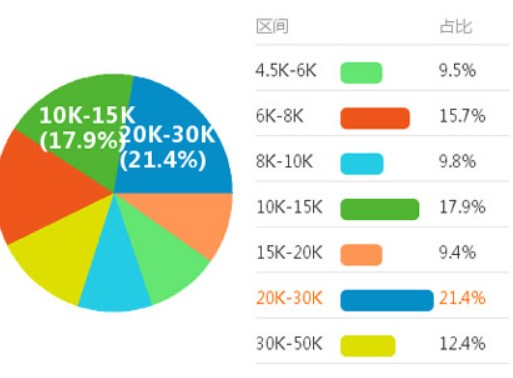
\includegraphics[keepaspectratio,width=200pt]{price.jpg}
    \caption{硬件工程师薪资(数据来源:职友集)}
\end{figure}

在大城市落脚不是一件容易的事,拿深圳为例,用于上下班的通勤可能就要花1小时
以上,初来乍到的自己也没有任性的资本,再加上受疫情影响,就业形势严峻,
能够找到一份稳定的工作就不是件容易的事,但抛开其他问题,深圳对于我来说不错的选择,
首先,深圳是一线城市对外地人较为友好的地方了,满足了年龄和学历的要求,就有了在深圳
安定的本钱。比起北上广,深圳是一个自然环境好、经济活力强、政府政策友好、融入
成本相对较低的城市。深圳房价是贵,但比起其他一线城市也算是中规中矩,
而且按照预想,我所希望的职位在深圳也有广泛的需求。在深圳湾科技园区,集中了腾讯、
阿里、百度、顺丰等互联网巨头,还有很多不明觉厉的本地巨头如大疆、
华大、OPPO、VIVO、中兴、TCL、康佳、迈瑞等高科技企业。

在一线城市,我想我会和其他人合租来减轻住房压力,
各项支出应该都不是一笔小数目,但因此所能够调动的资源也十分丰富,
作为硬件工程师,能够尽快获得自己所需的各项资源是一件不容忽略的事。
同时,选择大城市也是我的愿望,我希望能够在大城市丰富我的空闲时间,
在繁忙的工作中有更多可供选择的娱乐方式。

说完了可能面对的困难,不妨畅想一下一线城市丰富的生活。
深圳因为环境宜人,特别适合锻炼和散步。在这个全国公园最多的城市,
能够充分亲近自然,下班后可以爬个夜山,不拍晒黑又能在山顶看到
夜景。
\begin{figure}[htbp]
    \centering
    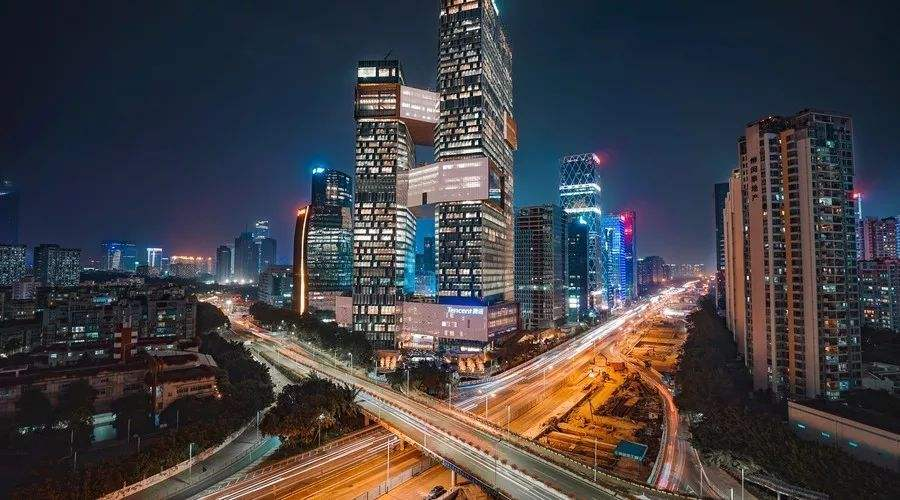
\includegraphics[keepaspectratio,width=300pt]{深圳生活.jpeg}
    \caption{深圳夜景}
\end{figure}

在假期的时候来一场远足,看看候鸟和红树林,
或者是驾车到大海边,享受内陆城市平日难以一览的风景。
在这里享受大城市的文化气息,和结交的朋友一起去逛展览,一起去
咖啡屋享受人生。

\section{近期的目标}
在大学本科毕业后,我想我会根据自己考研的结果判断是否继续读研还是进行就业,
因为自己所在的专业是电子信息基地班,我的目标职业是硬件工程师,
而这一职业所需的专业知识并不是一个小数目,需要庞大的知识体系去支持工作的开展,
而本科四年的学习也许不能满足这一需求,希望读研来完善自己的知识体系,站在一个
更好的平台去深造,在所查阅到的招募信息中,多数高薪职位也对学历有着要求。当然也可以在工作中
去丰富知识,这样可能会使自己在工作方面能够更加得心应手。

当然不能好高骛远,我预想中的未来生活,接下来的两年还是会在完成本科学习任务上展开,努力学习专业知识,例如微波技术、
接口技术等核心课程,加强动手实践的能力,真正地将知识运用到实际项目中,提高自己解决问题的能力。

\section{部分小结}
展望了未来毕业的生活,给自己的努力又多了一份理由,希望自己能够时刻鞭策自己,找准
道路,不要给自己找借口,努力改变自己能力弱的事实。

\chapter{尾声}
写到这里这篇成长史也就结束了,感谢您能够接受我那似抱怨搬的冗长的回忆和
近似幻想的美好未来展望,通过写这篇成长史,我的的确确是把从出生到现在的
人生经历又回忆了一遍,当我在码出自己的过往时,对自己又有了新的认识,相信
今后的自己会更有方向地在自己地道路上走下去。
\backmatter


% %=======%
% %引入参考文献文件
% %=======%
\bibdatabase{bib/POC}%bib文件名称 仅修改bib/ 后部分
\printbib
\nocite{*} %显示数据库中有的,但是正文没有引用的文献


% \Appendix

% 这里是附录页,可要可不要

% \Thanks.



\end{document}